\documentclass[conference]{IEEEtran}
\usepackage{graphicx}  % For images
\usepackage{listings}  % For code snippets
\usepackage{xcolor}  % For custom colors
\usepackage[utf8]{inputenc}
\usepackage{amsmath}
\usepackage{natbib} % For citations

% Citation aliasing
\defcitealias{saxena2020epie}{Saxena and Paul, 2020}
\defcitealias{agrawal-etal-2018-beating}{Agrawal et al., 2018}
\defcitealias{wible-tsao-2010-stringnet}{Wible and Tsao, 2010}

\lstset{
  basicstyle=\ttfamily,        % Set the basic style to a typewriter font
  breaklines=true,             % Enable line breaking
  frame=single,                % Frame the code block
  keepspaces=true,             % Keep spaces for indentation
  showstringspaces=false       % Do not replace spaces in strings with a specific character
}

\title{Leveraging Sequence Labeling for Idiomatic Expression Recognition in English Text}
\author{\IEEEauthorblockN{Aaron Pradhan}
	\IEEEauthorblockA{\today}}  % Date

\begin{document}

\maketitle

\begin{abstract}
Idiomatic expressions present a unique challenge in natural language processing, often requiring contextual understanding that goes beyond literal word meanings. This paper explores the development of machine learning models capable of distinguishing between idiomatic and literal usages of phrases within the English Possible Idiomatic Expressions (EPIE) dataset. Our approach combines traditional classifiers, such as Random Forest, Support Vector Machines, and Logistic Regression, with advanced sequence labeling techniques utilizing Bidirectional Long Short-Term Memory (BiLSTM) networks and Conditional Random Fields (CRF). We present a novel preprocessing pipeline that enhances tokenization and addresses the issue of unbalanced data through targeted oversampling and the optimization of model hyperparameters via dropout rate experiments. The paper's contributions are twofold: first, providing insights into the idiom classification task with a focus on formal idioms, and second, extending the methodology to sequence labeling that captures the nuanced placement of idiomatic expressions within text. Our findings indicate that while traditional classifiers offer a foundational understanding of idiomatic usage, sequence labeling models exhibit superior performance, particularly when fine-tuned with dropout regularization. The methodology and subsequent results underscore the significance of comprehensive preprocessing and the potential of sequence labeling models in the nuanced task of idiom identification.
\end{abstract}

\begin{IEEEkeywords}
Natural Language Processing, Idiom Identification, Machine Learning, Sequence Labeling, BiLSTM, CRF, Data Preprocessing.
\end{IEEEkeywords}

\section{Introduction}\label{sec:introduction}
Idiomatic expressions are a fundamental aspect of natural language, offering rich semantic meanings that often diverge from their literal interpretations. The automatic recognition of these expressions is crucial for a variety of applications, including machine translation, sentiment analysis, and natural language understanding. However, the task is complicated by the polysemous nature of language and the contextual nuances that dictate idiomatic usage. In this study, we employ the EPIE dataset \citepalias{saxena2020epie}, which distinguishes between idiomatic and literal usages of expressions, to train a model capable of sequence labeling for idiomatic expression recognition. Our approach is motivated by the limitations observed in idiom classification within the dataset, such as label inaccuracies and a scarcity of literal examples. Through a rigorous methodology that includes oversampling and cross-validation, we aim to build a model that not only serves as a benchmark for sequence labeling but also sheds light on the underlying challenges of idiom detection in computational linguistics.

\section{Dataset}

The study utilizes the English Possible Idiomatic Expressions (EPIE) dataset, which consists of 25,206 sentences featuring lexical instances of 717 idiomatic expressions from the Integrated Multi-dimensional Idiomatic Language (IMIL) dataset \citepalias{agrawal-etal-2018-beating}. These instances are harvested from the extensive StringNet database \citepalias{wible-tsao-2010-stringnet} through searches for the idiomatic expressions cataloged in the IMIL dataset. The EPIE corpus distinctly categorizes idioms into two types: static and formal.

Static idioms are invariant in their lexical composition, which enables their detection via straightforward string matching techniques. Conversely, formal idioms are subject to various lexical transformations, necessitating a more nuanced, supervised learning approach for accurate identification.

Each sentence in the EPIE dataset delineates:
\begin{itemize}
    \item The candidate idiom, such as "behind [pron] back" or "burn candles at both ends," which could manifest in multiple syntactic forms.
    \item The full sentence that provides context for the idiom's usage, punctuated in a manner that facilitates tokenization and subsequent analysis.
    \item A sequence of tags corresponding to each word or punctuation mark within the sentence. The tags follow a convention where "O" indicates a non-idiomatic segment, "B-IDIOM" marks the beginning of an idiomatic expression, and "I-IDIOM" denotes continuation of the idiom.
    \item Labels marked as either 0 or 1, exclusively associated with formal idioms, indicating whether the candidate phrase is employed idiomatically (1) or literally (0).
\end{itemize}

The EPIE authors describe the detection of idiomatic expressions as a sequence labeling task, advocating a dual-strategy approach to discern static from formal idioms. Our work predominantly leverages this structured dataset to construct models capable of sequence labeling, with an emphasis on the algorithmic discernment of idiomatic versus literal usages of expressions.

\section{Methodology}

\subsection{Dataset Preparation}
For idiom classification, we focused exclusively on the formal idioms subset, due to the presence of labels indicating idiomatic or literal usage. For sequence labeling, we included both static and formal idioms, benefiting from the comprehensive tagging provided for each sentence.

\subsection{Preprocessing}
The preprocessing pipeline was designed to maintain the integrity of the idiomatic expressions. This involved lowercasing the text while retaining stopwords and punctuation, as they are critical for understanding the structure and meaning of idiomatic phrases. For sequence labeling, sentence lengths were analyzed, and we chose to truncate to 100 words based on the 99th percentile of the length distribution to mitigate the inclusion of atypically long transcriptions.

\begin{figure}[htbp]
\centerline{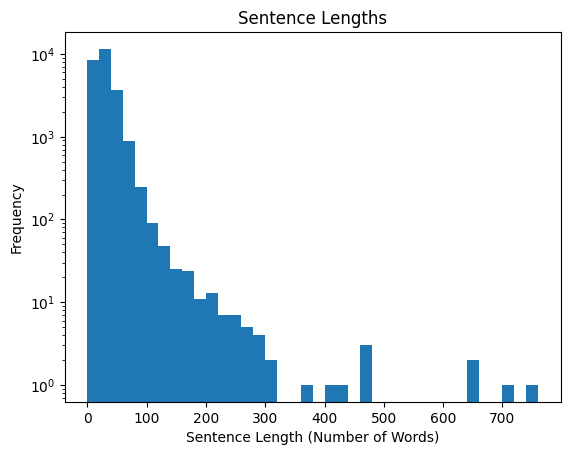
\includegraphics[width=0.5\textwidth]{fig_sentence_length_distribution.png}}
\caption{Distribution of sentence lengths in the EPIE dataset.}
\end{figure}

\subsection{Tagging for Sequence Labeling}
The tagging approach was simplified by unifying 'B-IDIOM' and 'I-IDIOM' into a single 'I-IDIOM' tag, corresponding to class `2`, thereby streamlining the model's task to differentiate idiomatic from non-idiomatic sequences without additional start-of-idiom complexity.

\subsection{Refined Preprocessing for Sequence Labeling}
Further preprocessing was performed after preliminary model results. Specifically, we zeroed out tags for negative samples to align the input data with their literal meaning. Additionally, tokenization was refined to address issues with special characters, ensuring they were treated as separate tokens to maintain the integrity of idiomatic expressions.

\subsection{Model Selection}
For idiom classification, traditional machine learning models such as Support Vector Machine (SVM), Random Forest (RF), and Logistic Regression (LR) were employed. These models were chosen for their ability to establish baseline performance across different decision-making strategies.

\subsection{Model Training for Idiom Classification}
The idiom classification models were trained using the formal idioms subset. The RandomOverSampler method was applied to address the class imbalance present within the dataset, ensuring an equal distribution of idiomatic and literal usage samples during training.

\subsection{Model Architecture for Sequence Labeling}
The sequence labeling model consisted of the following architecture, designed to capture the sequential dependencies of idiomatic language:
\begin{lstlisting}[language=Python]
input_tensor = Input(shape=(max_len,))
model = Embedding(input_dim=len(word_tokenizer.word_index) + 1,
                  output_dim=50, input_length=max_len)(input_tensor)
model = Bidirectional(LSTM(units=100, return_sequences=True,
                  recurrent_dropout=0.1))(model)
model = TimeDistributed(Dense(50, activation="relu"))(model)
crf = CRF(len(tag_tokenizer.word_index) + 1)
out = crf(model)
model = ModelWithCRFLoss(Model(input_tensor, out))
model.compile(optimizer="adam")
\end{lstlisting}
This architecture, comprising an embedding layer, a bidirectional LSTM, and a CRF layer, is particularly well-suited for sequence labeling tasks. The bidirectional LSTM captures context from both directions, which is crucial for understanding the nuanced usage of idiomatic expressions. The CRF layer enhances the model's ability to make coherent sequence-level predictions, essential for the correct labeling of idiomatic phrases.

\subsection{Ablation Studies}
We systematically ablated components of our sequence labeling model to investigate their impact on performance.

\textbf{BiLSTM with CRF Layer}: We began by evaluating the effect of LSTM unit variations within our BiLSTM model complemented by a CRF layer. This model serves as our baseline, and we experimented with 50, 100, and 200 LSTM units to observe the changes in model performance. The LSTM units are a crucial hyperparameter, determining the model's capacity to capture dependencies within the data. Our hypothesis was that increasing the number of units would allow the model to capture more complex patterns, but also risk overfitting.

\textbf{BiLSTM without CRF Layer}: To assess the CRF layer's contribution, we compared the baseline model against a BiLSTM network sans the CRF layer, maintaining 100 LSTM units for consistency. The CRF layer typically enhances the model's ability to make structured predictions, which is beneficial in sequence labeling tasks. Removing the CRF layer allowed us to discern its specific impact on the overall performance.

\textbf{BiLSTM with Dropout Layer}: Recognizing the potential for overfitting, we incorporated a dropout layer into the BiLSTM architecture with 50 LSTM units, given its smaller parameter space less prone to overfitting. We experimented with dropout rates ranging from 0.1 to 0.5, in increments of 0.1. Dropout is a regularization technique that randomly deactivates a fraction of neurons during training, promoting the development of more robust features by preventing co-adaptation.

Each ablation configuration was rigorously trained and validated to ensure consistent comparison. The ablation results provided insights into the importance of each component and guided the optimization of our final model for the sequence labeling task.

\section{Results}

\subsection{Idiom Classification Results}
In the idiom classification task, we evaluated three machine learning models: Random Forest (RF), Support Vector Machine (SVM), and Logistic Regression (LR). These models were chosen for their capacity to offer a diverse range of decision-making strategies and their suitability for baseline performance establishment.

The SVM and LR models demonstrated a high degree of accuracy, with the SVM slightly outperforming LR. The RF model, while also displaying high accuracy, showed a more significant standard deviation in precision, which may indicate variability in performance across different test sets or data partitions.

Confusion matrices for the three models provided deeper insight into their classification behavior:
\begin{verbatim}
Confusion Matrix for Random Forest:
[[ 10  66]
 [  4 548]]

Confusion Matrix for SVM:
[[  3  73]
 [  1 551]]

Confusion Matrix for Logistic Regression:
[[  2  74]
 [  0 552]]
\end{verbatim}

These matrices reveal that while all models were proficient in classifying the majority class (true negatives and true positives), they struggled more with correctly identifying the minority class (false negatives and false positives), a common challenge in imbalanced datasets.

The overall scores for the models were as follows:
\begin{verbatim}
Random Forest Scores:
accuracy: Mean=0.89, Std=0.00
precision_macro: Mean=0.83, Std=0.08
recall_macro: Mean=0.54, Std=0.01
f1_macro: Mean=0.54, Std=0.02

SVM Scores:
accuracy: Mean=0.89, Std=0.00
precision_macro: Mean=0.80, Std=0.04
recall_macro: Mean=0.53, Std=0.01
f1_macro: Mean=0.53, Std=0.02

Logistic Regression Scores:
accuracy: Mean=0.87, Std=0.02
precision_macro: Mean=0.68, Std=0.04
recall_macro: Mean=0.66, Std=0.03
f1_macro: Mean=0.67, Std=0.04
\end{verbatim}

The RF model showed the highest precision, indicating its effectiveness at correctly identifying positive instances when it predicted them. However, its recall was comparable to the SVM, suggesting a difficulty in capturing all positive instances. Logistic Regression displayed a more balanced performance between precision and recall, as reflected in its f1\_macro score.

\subsection{Sequence Labeling Results}

\subsubsection{LSTM Unit Sizes Ablation Study}

The sequence labeling task was addressed with LSTM models of varying unit sizes, specifically 50, 100, and 200 units. Across different configurations, the models achieved high precision and recall for both non-idiom words (Class 1) and padding tokens (Class 0). However, the identification of idiomatic expressions (Class 2) presented a greater challenge, as evidenced by the lower F1-scores in this category. Notably, the LSTM model with 50 units attained an F1-score of 0.78 for idiomatic expressions, which, while lower than the other classes, still represents a significant achievement given the complexity of the task. The LSTM models with 100 and 200 units did not significantly outperform the 50-unit model, suggesting that increasing the number of units does not necessarily correlate with higher performance for this dataset and task.

The classification reports for these LSTM models are as follows:
\begin{table}[ht]
\centering
\small
\caption{Classification report for the LSTM model with 50 units}
\begin{tabular}{ccccr}
\hline
Class & Precision & Recall & F1-Score & \multicolumn{1}{c}{Support} \\
\hline
0 (Padding) & 0.99 & 1.00 & 0.99 & 358971 \\
1 (Non-idiom) & 0.97 & 0.95 & 0.96 & 127119 \\
2 (Idiom) & 0.80 & 0.76 & 0.78 & 14510 \\
\hline
Accuracy & & & 0.98 & 500600 \\
Macro Avg & 0.92 & 0.90 & 0.91 & 500600 \\
Weighted Avg & 0.98 & 0.98 & 0.98 & 500600 \\
\hline
\end{tabular}
\label{tab:classification_report_lstm_50_units}
\end{table}

\begin{table}[ht]
\centering
\small
\caption{Classification report for the LSTM model with 200 units}
\begin{tabular}{lcccc}
\hline
Class & Precision & Recall & F1-Score & Support \\
\hline
0 (Padding) & 0.99 & 1.00 & 0.99 & 358971 \\
1 (Non-idiom) & 0.97 & 0.95 & 0.96 & 127119 \\
2 (Idiom) & 0.79 & 0.77 & 0.78 & 14510 \\
\hline
Accuracy & & & 0.98 & 500600 \\
Macro Avg & 0.92 & 0.90 & 0.91 & 500600 \\
Weighted Avg & 0.98 & 0.98 & 0.98 & 500600 \\
\hline
\end{tabular}
\label{tab:classification_report_lstm_200_units}
\end{table}

(The classification report for the LSTM model with 100 units was exactly the same as the report for the model with 200 units, so it has been omitted.)

\subsubsection{Dropout Ablation Study}
In the sequence labeling task, the LSTM models with different dropout rates were evaluated. The dropout rate is a hyperparameter that dictates the proportion of neurons to drop during the training process, to prevent overfitting.

The validation loss graph and classification reports for dropout rates of 0.1, 0.2, 0.4, and 0.5 indicate the following:

\begin{itemize}
\item Dropout Rate 0.1: Achieved the best balance between precision, recall, and F1-score for idiomatic expressions, with the validation loss decreasing steadily across epochs.
\item Dropout Rate 0.2: Showed similar performance to a dropout rate of 0.1, suggesting that a slight increase in regularization does not substantially impact the model's ability to generalize.
\item Dropout Rate 0.4 and 0.5: As the dropout rate increased, the precision and F1-score for idiomatic expressions slightly decreased, indicating that excessive regularization may hinder the model's learning capability.
\item Dropout Rate 0.3: Exhibited a significant drop in performance, with precision and recall for idiomatic expressions falling to 0. This anomaly suggests that a dropout rate of 0.3 may be too aggressive for the network architecture and dataset, leading to underfitting.
\end{itemize}

These findings underscore the importance of tuning dropout rates to match the dataset and model architecture. While moderate dropout rates (0.1-0.2) aid in generalization without sacrificing performance, higher rates may lead to a degradation in the model's ability to identify idiomatic expressions accurately.

\begin{figure}[htbp]
\centerline{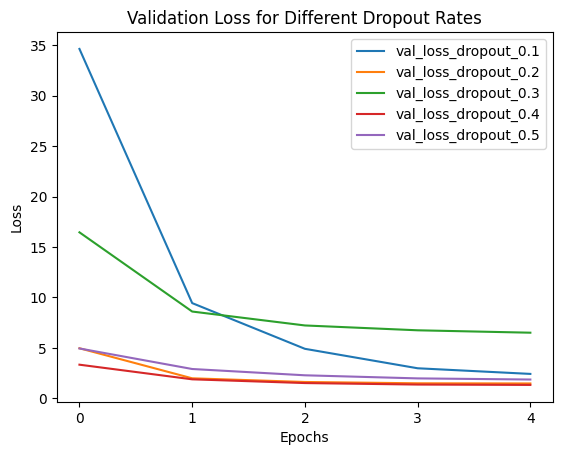
\includegraphics[width=0.5\textwidth]{val_loss_for_dropout_rates.png}}
\caption{Validation losses for different dropout rates.}
\end{figure}

\subsection{Impact of Preprocessing Adjustments}
The additional preprocessing steps, such as zeroing out tags for negative samples and refining tokenization, played a crucial role in the performance enhancement observed in the sequence labeling models. These adjustments facilitated the models' ability to more accurately tag idiomatic expressions and align with the expected sequence labels, as evidenced by the manual inspection and analysis of the predictions.

\subsection{Discussion}
The results from the idiom classification and sequence labeling tasks underscore the intricate balance between model complexity and data quality. While advanced models with a higher number of LSTM units did not necessarily yield better results, the refinement of preprocessing steps notably improved model performance, particularly for the sequence labeling task. This emphasizes the importance of careful data preparation and the potential of even relatively simple models to achieve high accuracy when optimally configured and trained.

\section{Future Work}

The exploratory nature of this research opens several avenues for future investigation. A comparative analysis between the performance metrics for formal and static idioms presents a compelling direction. Such a study would entail a granular examination of the accuracy, precision, recall, and other relevant metrics to delineate the challenges unique to each idiom type.

Further work could also investigate the integration of context-aware algorithms that leverage larger linguistic units than individual sentences, aiming to capture the broader discourse within which idiomatic expressions function. Additionally, expanding the corpus to include a more diverse set of idiomatic expressions could improve the robustness and generalizability of the models.

Another promising area of future research lies in the application of deep learning techniques, particularly transformer-based architectures like BERT and GPT, which have demonstrated exceptional performance in understanding context and semantics in text. Fine-tuning such models on the idiom detection task could yield improvements, especially in discerning the subtle nuances that differentiate idiomatic from literal usage.

Moreover, the incorporation of unsupervised and semi-supervised learning methods could provide insights into the idiomatic phenomena that are not well-represented in the current dataset. This could also help in addressing the mislabeling issue identified in the manual error analysis, potentially leading to the creation of a more accurate and comprehensive idiom-labeled dataset.

Finally, cross-linguistic studies that apply the developed models to idiomatic expressions in other languages could contribute to the field of cross-cultural natural language understanding and the development of more sophisticated multilingual NLP systems.

\section{Conclusion}

This research aimed to classify idiomatic expressions in English text using the EPIE dataset. Initial model training with traditional classifiers established baseline performances, while subsequent experiments with LSTM and CRF layers focused on sequence labeling tasks. The study revealed that adjustments in preprocessing steps and tokenization were critical in improving the model's ability to recognize idiomatic expressions, particularly in a dataset marked by class imbalances.

The findings suggest that the complexity of natural language idioms poses significant challenges for classification models, which require careful consideration of data preparation and model architecture. Although increasing LSTM units did not lead to performance gains, the nuanced sequence labeling approach did show promise in identifying non-idiomatic tokens with high accuracy.

Future efforts will explore comparative analyses of idioms, additional model architectures, and advanced embeddings to further enhance performance. This research serves as a foundation for more sophisticated natural language processing applications capable of understanding the nuanced usage of language.


	\bibliographystyle{IEEEtran}
	\bibliography{references}

\end{document}
